¿Qué modificación harías en el diagrama de la figura a), sin perder información, para que se puedan conocer qué alumnos toman clase cada profesor?
\begin{center}
    
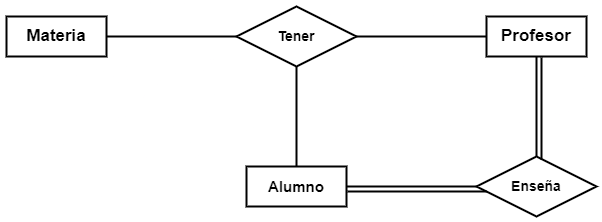
\includegraphics[width=10cm]{resources/2.2.png}
\end{center}
Agregamos una relación binaria entre Profesor y Alumno que nos ayuda a no perder información y garantizar que podemos saber qué alumnos toman clase con cada profesor ya que conoceríamos a qué alumnos les enseña. 